%%%%%%%%%%%%%%%%%%%%%%%%%%%%%%%%%%%%%%%%%%%%%%%%
% COPYRIGHT: (C) 2012-now FAU FabLab and others, CC-BY-SA 3.0
%%%%%%%%%%%%%%%%%%%%%%%%%%%%%%%%%%%%%%%%%%%%%%%%


\newcommand{\basedir}{fablab-document}
\documentclass{\basedir/fablab-document}

% \usepackage{fancybox} %ovale Boxen für Knöpfe - nicht mehr benötigt
\usepackage{amssymb} % Symbole für Knöpfe
\usepackage{subfigure,caption}

\usetikzlibrary{shapes,arrows} % für das flowchart

\usepackage{marvosym} % für Briefumschlag-Symbol
\usepackage{eurosym}
\usepackage{tabularx} % Tabellen mit bestimmtem Breitenverhältnis der Spalten
\usepackage{multirow} % Tabellen Zellen die sich über mehrere Zeilen ausdehnen
\usepackage{wrapfig} % Textumlauf um Bilder
\renewcommand{\texteuro}{\euro}

\linespread{1.2}
\fancyfoot[L]{kontakt@fablab.fau.de}
\title{Einweisung Lasercutter}

\tikzstyle{laserknopf} = [anchor=base, draw=black, fill=gray!10, rectangle, rounded corners, inner sep=2pt, outer sep = 3pt]
\tikzstyle{lueftungsknopf} = [anchor=base, color=white, draw=black, fill=gray, rectangle, rounded corners, inner sep=2pt, outer sep = 3pt]

% styles für das Flowchart
\tikzstyle{decision} = [diamond, draw, fill=blue!20,
    text width=4.5em, text badly centered, node distance=3cm, inner sep=0pt]
\tikzstyle{block} = [rectangle, draw, fill=blue!20,
    text width=5em, text centered, rounded corners, minimum height=4em]
\tikzstyle{line} = [draw, very thick, color=black!50, -latex']
\tikzstyle{cloud} = [draw, ellipse,fill=red!20, node distance=3cm,
    minimum height=2em]

% Knöpfe für Laser und Fernbedienung
\newcommand{\knopf}[2]{
    \begin{tikzpicture}[baseline={(box.base)}]
    \node [#1] (box) {
        \fontsize{9pt}{9pt}\selectfont \textbf{#2}\strut
    };
    \end{tikzpicture}
}


\renewcommand{\todo}[1]{\textbf{\color{red}{TODO: #1}}}


%\newcommand{\laserKnopf}[1]{\,\Ovalbox{\fontsize{9pt}{9pt}\selectfont \textbf{#1}}\ }
\newcommand{\laserKnopf}[1]{\knopf{laserknopf}{#1}}
\newcommand{\laserZingXyAus}{\laserKnopf{X/Y aus}}
\newcommand{\laserRoterLaser}{\laserKnopf{roter Laser}}
\newcommand{\laserZingStart}{\laserKnopf{Start}}
\newcommand{\laserZingStop}{\laserKnopf{Stop}}
\newcommand{\laserZingReset}{\laserKnopf{Reset}}
\newcommand{\laserLTTPause}{\laserKnopf{$\blacktriangleright\,\parallel$}} % TODO: schöneres Pause-Symbol suchen
\newcommand{\laserLTTStop}{\laserKnopf{$\square$}}
\newcommand{\laserJob}{\laserKnopf{Job}}
\newcommand{\laserFocus}{\laserKnopf{Focus}}
\newcommand{\laserPfeilRauf}{\laserKnopf{$\blacktriangle$}}
\newcommand{\laserPfeilRunter}{\laserKnopf{$\blacktriangledown$}}


\newcommand{\laserDisplay}[1]{\fbox{\texttt{#1}}}

\newcommand{\lueftungKnopf}[1]{\knopf{lueftungsknopf}{#1}}
%der echte Enterpfeil geht leider nicht: \newcommand{\lueftungEnter}{\lueftungKnopf{↲}}
% stattdessen ein gespiegelter Pfeil ↰, der fast genauso aussieht.
\newcommand{\reflectboxX}[1]{\raisebox{\depth}{\scalebox{1}[-1]{#1}}} % Spiegelung an x-Achse
\newcommand{\returnSymbol}{\reflectboxX{\ensuremath{\mathbf{\Lsh}}}} % Enterpfeil (sieht fast genauso aus)
\newcommand{\lueftungEnter}{\lueftungKnopf{\returnSymbol}}

%\newcommand{\lueftungEnter}{\lueftungKnopf{\ensuremath{\mathbf{\hookleftarrow}}}}
\newcommand{\lueftungMinus}{\lueftungKnopf{-}}
\newcommand{\lueftungPlus}{\lueftungKnopf{+}}
\newcommand{\lueftungOn}{\lueftungKnopf{On}}
\newcommand{\lueftungOff}{\lueftungKnopf{Off}}
\newcommand{\lueftungPfeilRauf}{\lueftungKnopf{$\blacktriangle$}}
\newcommand{\lueftungPfeilRunter}{\lueftungKnopf{$\blacktriangledown$}}


%VisiCut Buttons
\newcommand{\button}[1]{\knopf{lueftungsknopf}{#1}} %TODO

\newcommand{\pfeil}{\ensuremath{\rightarrow}}

\newcommand{\nurZing}{\emph{nur für Epilog Zing:} }
\newcommand{\nurLTT}{\emph{nur für LTT iLaser:} }

\begin{document}
\maketitle

Diese Einweisung erklärt die Lasercutter LTT iLaser 4000 (seit Sept. 2018 im FAU FabLab) und Epilog Zing (kleiner, Vorgänger, aus Platzmangel normalerweise nicht im FabLab).

\todo{Achtung, die Erklärungen sind oft nur für den Zing und noch nicht für den neuen LTT! Daher ist es noch nicht möglich, eine Einweisung in den LTT-Laser zu erhalten. Sobald alles passt, bitte diesen Hinweis entfernen.}

\section{Was du dir merken musst}
Den Inhalt dieses Kapitels musst du wissen, alles andere kannst du bei Bedarf nachlesen.
\subsection{Regeln und Hinweise}
\begin{itemize}
 \item Nur zweifelsfrei geeignete Materialien verwenden, die in der Liste (auf den nächsten Seiten) stehen. Keine unbekannten Materialien, kein PVC, Teflon, etc.
 \item Ebenfalls nicht erlaubt sind leichtentzündliche oder gefährliche Dinge, wie z.\,B. gefüllte Feuer\-zeuge. Wenn das Gehäuse nicht aus Metall ist, muss bei Handys der Akku herausgenommen werden.
 \item Lasercutter nur unter ständiger Beobachtung betreiben! Solange der Laser aktiv ist, muss immer eine Person \emph{direkt} beim Lasercutter sein. Für vollständig unbrennbare Materialien (Glas, nicht lackierte Metallteile) gibt es eine Ausnahme, wenn vorher alle brennbaren Reste aus dem Schneidetisch entleert wurden.
 \item Alle Arbeiten erfolgen auf eigenes Risiko, auch wenn dein schickes Handy beim Gravieren kaputtgeht.
 \item Die Schrauben zur Befestigung des Schneidetischs (Wabengitter) dürfen gedreht werden, ansonsten nichts schrauben oder verstellen. \todo{Diese durch Rändelschrauben ersetzen, um Verwechslungen zu vermeiden, und grün markieren (z.\,B. Plotterfolie um die Soll-Position) damit wir den gleichen Text wie beim Zing verwenden können}
 \item \nurZing Die grün markierten Rändelschrauben am Schneidetisch dürfen von Hand gedreht werden, ansonsten nichts verstellen. % Betätigen der grünen Schrauben ist nötig, um den Schneidetisch zu reinigen! Deshalb kann man es nicht ganz verbieten.
 \item Im Brandfall nur mit CO\subscript{2}-Löscher, niemals mit Pulver-, Schaum- oder Wasserlöscher löschen (Verschmutzung, Stromschlaggefahr)! Der Feuerlöscher steht direkt neben dem Lasercutter.
 \item \nurLTT \todo{...}
 \item \nurLTT Sofortiges Abschalten des Lasercutters geht nur mit dem Not-Aus-Schalter. \laserLTTPause fährt die aktuellen Linien noch zu Ende!
 \item \nurZing Es gibt keinen Not-Aus-Schalter! \laserZingStop  fährt die aktuelle Linie noch zu Ende. Sofortiges Abschalten des Lasercutters geht nur über den Kippschalter rechts unten am Gerät.
\end{itemize}

% Messing ist nicht verboten, auch wenn es nicht geht, denn dieser Laser hat einen Schutz gegen Reflektionen (Aussage des Zing-Technikers, auf explizite Frage, was passiert, wenn ich den Strahl 100% spiegle und in den Laser zurückwerfe, ähnliche-Aussage des LTT-Vertrieblers)
\pagebreak % lieber hier ein Seitenumbruch, anstatt den nächsten Punkt zu zerreißen
\subsection{Bei kleineren Flammen}
Eine \emph{kleinere} Flamme am Laserpunkt und leichter Geruch kann manchmal auftreten:
\begin{itemize}
 \item Zum Pausieren \laserLTTPause (\nurZing \laserZingStop) drücken: Druckauftrag wird \emph{nach} dem Ende der aktuellen Linie pausiert. Bis zum Anhalten kann es unter Umständen lange dauern!
 \todo{\nurLTT manchmal reagiert der Laser auch bei Visicut nicht auf Pause, als hätte er den Tastendruck nicht mitbekommen, auch wenn es später die Möglichkeit zur Pause gäbe. Unklar, wann und wieso.}
 \item Sicherstellen, dass die Absaugung angeschaltet ist und Air Assist (Druckluft bei der Linse) an ist.
 \item Bei manchem Material lässt es sich nicht vermeiden und dann ist es auch nicht weiter schlimm.
\end{itemize}

\subsection{Im Ernstfall}
Bei \emph{größeren} Flammen oder starker Rauchentwicklung muss das Lasern \emph{sofort} unterbrochen werden, da sonst die Linse beschädigt wird:
\begin{itemize}
 \item \textbf{Deckel leicht öffnen} (Laser wird ausgeschaltet, der Antrieb fährt jedoch weiter).\\
 \nurLTT Oder auch den Not-Aus betätigen.
 \item \textbf{Betreuer rufen}
 \item Letzter Ausweg ist das Löschen mit dem CO\subscript{2}-Löscher in kurzen Sprühstößen. Ein Feuerlöscher befindet sich beim Kassenterminal gleich gegenüber vom Lasercutter, sowie am Durchgang zur Elektrowerkstatt.
 \item Bei weiterer Eskalation die Feuerwehr rufen, anwesende Personen warnen und den Raum verlassen (Erstickungsgefahr durch CO\subscript{2} und durch Rauch)
\end{itemize}


\subsection{Wieso muss ich immer beim Lasern dabeibleiben?}
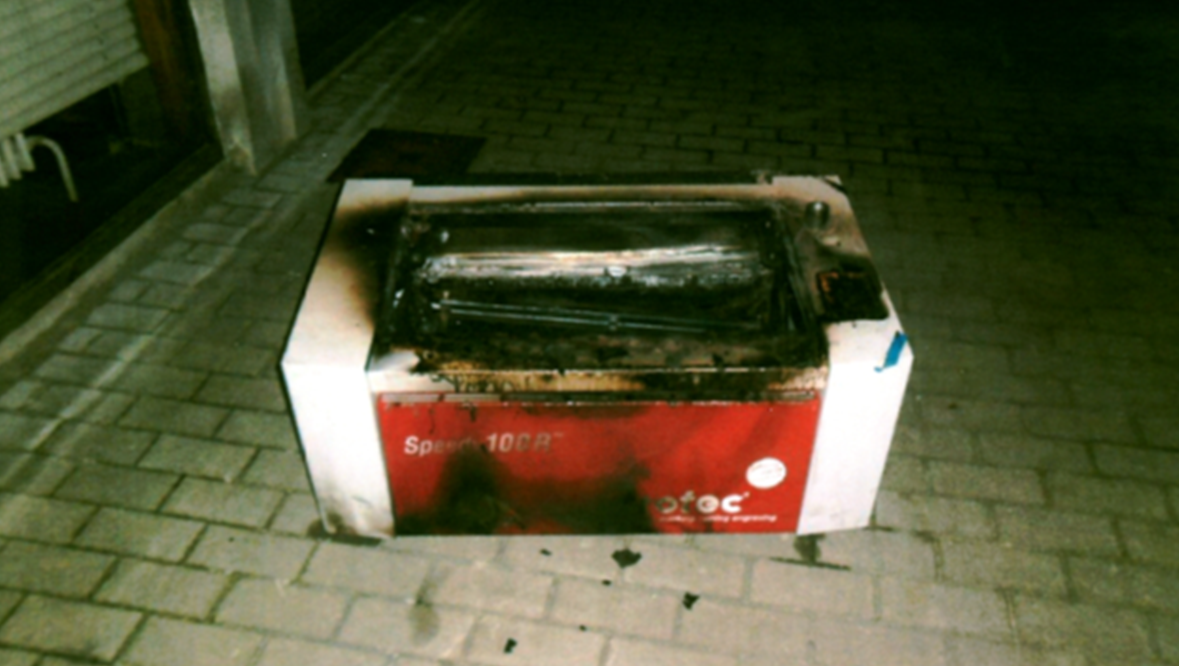
\includegraphics[width=.75\linewidth]{./img/laser-abgebrannt_fablab_leuven.jpg}
% Mit freundlicher Erlaubnis von Marc Lambaerts, KU Leuven

Bild: Ein ausgebrannter Lasercutter des FabLab Leuven. Der Benutzer meinte, weil die Datei dreimal funktioniert hat, müsse man beim vierten mal nicht mehr dabeibleiben.


\vspace{5em}
\hrule

Alles bis hier musst du auswendig wissen. Den Rest kannst du bei Bedarf nachschauen.
\vspace{0.2em}
\hrule
\vspace{3em}

\section{Materialien}
Wenn ein Material nicht zweifelsfrei erlaubt ist, frage unbedingt nach! Viele Kunststoffe sehen gleich aus, und Baumärkte haben schon oft falsche Sorten verkauft, weshalb Kunststoff ohne Beschriftung im Zweifelsfall nicht gelasert werden darf.

\subsection{Erlaubt}
\newcommand{\itemCheck}{\item[\checkmark]}
\begin{itemize}
\itemCheck unbrennbares zum Gravieren: Metall, Glas, Keramik, Stein
\itemCheck dünne Lackschichten auf Metall (außer Teflonbeschichtung)
\itemCheck erlaubte Kunststoffe: Acrylglas (PMMA), PET (Overheadfolie, Bayer Vivak), Moosgummi (EVA-Schaum)
\itemCheck Holz, Pappe, Papier und Ähnliches (HDF, Butterkeks ohne Schokolade, Brezen, ...)
\itemCheck PE Polyethylen: Schaumstoffe gehen gut, Platten schlecht laserbar aber trotzdem erlaubt
\itemCheck PS Polystyrol bis 1mm Dicke
\itemCheck PC Polycarbonat bis 1mm Dicke
\itemCheck spezieller laserbarer Stempelgummi aus dem FabLab
\itemCheck Heißlaminierfolie \emph{nur} wenn sie laut Datenblatt des Herstellers aus PET+EVA besteht\\(keine Kaltlaminierfolie, diese enthält oft PVC!) 
\end{itemize}

\subsection{Verboten}
\newcommand{\itemCross}{\item[$\times$]}
\begin{itemize}
\itemCross im Zweifelsfall: alles was nicht erlaubt ist
\itemCross nicht eindeutig identifizierbare Kunststoffe (\enquote{irgendwas durchsichtiges})
\itemCross spritzendes oder stark wässriges Material (Schokolade, ...)
\itemCross ABS, Epoxidharz (GFK, CFK, Platinen), weil es übelst stinkt
\itemCross PS Polystyrol / PC Polycarbonat dicker als 1\,mm, weil es beim Lasern spritzt
\itemCross halogenhaltige Kunststoffe: PVC = Vinyl = Neopren, PTFE = Teflon (z.\,B. als \enquote{glitschige} Beschichtung von Taschenmessern), PFA, ...
\end{itemize}

\section{Grundlagen}
Der Lasercutter hat zwei Laser: Einen roten Laserpointer, der weitestgehend harmlos ist. Dieser ist wie ein Laserpointer ungefährlich, solange man den direkten Strahl (z.\,B. mit einem Spiegel) höchstens für sehr kurze Zeit betrachtet. Das Betrachten des roten Punkts auf einem Objekt ist harmlos.

Der eigentliche Laser (Infrarot mit hoher Leistung) wird sofort abgeschaltet, wenn Schutzscheibe oder Frontklappe geöffnet sind. Von ihm geht keine Gefahr aus, solange die Schutzschalter nicht manipuliert werden. Daher: keine Magneten an der Vorder- und Oberseite des Lasercutters anbringen.

\section{Datei erstellen}
Lege mit einem Vektorzeichenprogramm (Inkscape, Corel Draw, Adobe Illustrator) die Datei an. Je nach Programm unterscheidet sich das Vorgehen etwas:

% TODO VisiCut + Illustrator/Corel beschreiben?

\subsection{Inkscape + VisiCut (empfohlen)}
Wenn du Inkscape verwendest, wähle möglichst folgende Aufteilung, damit du es direkt in VisiCut weiterverarbeiten kannst.

\textbf{Schneiden}: Pfade mit Linienfarbe rot, Liniendicke ist egal, keine Füllung.

\textbf{Gravur}: Schwarz, Graustufen, oder beliebige Pixelgrafiken (Fotos).

\textbf{Linie markieren}: Linienfarbe grün, keine Füllung.

\textbf{Kommentare}: Linienfarbe oder Füllung blau. So kannst du z.\,B. Erklärungstexte mit in deine Datei einbauen, die nicht gelasert werden sollen.

Bringe die Datei als SVG mit. Wenn du Schriftarten verwendest, die wir im FabLab nicht installiert haben, wandle den Text in Pfade um.

%Du kannst VisiCut auch auf deinem eigenen Rechner installieren.

\subsection{Corel Draw, Adobe Illustrator, ... + VisiCut}
\label{corel-illustrator-svg-visicut}
Verfahre wie bei Inkscape beschrieben, und zusätzlich:

\begin{itemize}
\item Setze den Farbraum auf RGB: zu schneidende Linien müssen echtes RGB-rot (255,0,0) sein.
\item Wandle Text in Pfade um
\item Corel: Beim SVG-Export die Einstellung \enquote{Formoptionen = Darstellungsattribute} setzen.
\end{itemize}

Dieses Vorgehen könnte in Zukunft einfacher werden, wenn ein Visicut-Plugin für Corel oder Illustrator fertigentwickelt wird. Wenn du daran mit entwickeln möchtest, um das Vorgehen genauso einfach zu machen wie bei Inkscape, melde dich bei uns.

\subsection{Corel Draw, Adobe Illustrator, sonstiges + Windows-Druckertreiber}
Als Seitengröße sollten die Maße des Schneidtisches gewählt werden (1000 $\times$ 600~mm / \nurZing 609\,$\times$\,304~mm), da sonst Probleme auftreten können.

\textbf{Vektor (Schneiden)}: Zu schneidende Linien auf eine Linienbreite von höchstens 0,001 inch stellen (Inkscape: 0,1 px, Corel Draw: Haarline, Adobe Illustrator: 0,1 px, Vectorworks: 0,03 mm). Bei fertigen Zeichnungen aus dem Internet ist Vorsicht geboten, manchmal sind hinter gefüllten Flächen solche dünnen Linien versteckt, die dann durchgeschnitten werden.

\textbf{Raster (Gravur)}: Alles, das keine dünne Vektorlinie ist (sicher ab 0,25mm / 0,008 inch), wird graviert, sowohl dicke Linien und Flächen als auch Pixelgrafiken (Fotos). Die Gravur erfolgt im Graustufenmodus, sodass hellere Flächen nur leicht graviert werden, schwarze Flächen jedoch vollständig.

Dokument als PDF (oder Corel CDR) auf Windows-Freigabe ablegen. Beim Speichern einen aussagekräftigen Namen wählen, da dieser später auf dem Display erscheint.

\section{Job senden}

\subsection{VisiCut (empfohlen)}
\label{VisiCut}

Aus Inkscape kann man direkt über ein Plugin die markierten Zeichnungen in VisiCut exportieren. Dazu klickt man in Inkscape auf \button{Erweiterungen} / \button{Lasercut Path} %TODO in Illustrator auf ....
. Bei Illustrator/Corel muss man ein SVG exportieren wie in \ref{corel-illustrator-svg-visicut} beschrieben und dieses direkt mit Visicut öffnen.

Anschließend kann man rechts folgende Einstellungen treffen:

\textbf{Material}: In der oberen Dropdown Box kann das gewünschte Material ausgewählt werden.

\textbf{Stärke (mm)}: In der Dropdown Box kann die Dicke des Materials ausgewählt werden.

Für jede Stärke von jedem Material speichert Visicut Lasereinstellungen. Größtenteils sind diese bereits auf sinnvolle Werte eingestellt.

\textbf{Fokus}:

\nurLTT Ändern des Fokus wird in Visicut noch nicht unterstützt. Der Fokus wird immer auf die Material-Oberseite gesetzt, dazu einfach den Autofokus ausführen.

\nurZing Ein besonderes Feature ist, dass man den Fokus nicht verstellen muss, wenn man ihn auf die Grundplatte gesetzt hat, da VisiCut aus zu jedem Material den optimalen Fokus speichert und ihn automatisch anfährt. Dies kann man ausschalten, wenn man den Haken rechts bei \enquote{Fokus ist anfangs auf der Grundplatte...} heraus macht.

\textbf{Mapping}: Im Bereich Mapping kann man auswählen, wie entschieden werden soll, was geschnitten, graviert und markiert wird. Die Unterscheidung kann nach verschiedenen Kriterien erfolgen; standardmäßig wird nach Farbe entschieden: \enquote{schneide rot, graviere Rest, ignoriere blau, markiere grün}.

%TODO Position

\textbf{Laser Einstellungen}: Im Bereich Laser Einstellungen können die Lasereinstellungen überprüft und verstellt werden. Überprüfe vor Allem wenn es sich um ausgefallenere Materialien handelt, ob hier sinnvolle Einstellungen stehen. Oft ist es so, dass die Standardeinstellungen (Power: 0, Speed: 100, Fokus 0) gesetzt sind da diese noch nicht angepasst wurden). \textbf{Speichere deine Veränderungen nur, wenn sie auch für andere Benutzer sinnvoll sind.} Experimente bitte nicht abspeichern, sondern einfach nur den Auftrag abschicken ohne auf Speichern zu klicken.

\button{Berechnen}: Dadurch wird die benötigte Zeit im Vorraus berechnet. Dies ist allerdings nur ein Richtwert und kann von der tatsächlichen Dauer abweichen.

\button{Ausführen}: Dies schickt den Auftrag an den Lasercutter. Wenn eine Erfolgsmeldung erscheint, kann der Auftrag im Laser gestartet werden.

Da VisiCut in Java programmiert ist, läuft es auf jedem Betriebsystem und man kann es auch bei sich auf den Laptop installieren. Es ist verfügbar unter \url{https://download.visicut.org/}.

Die aktuell verwendet Konfiguration für VisiCut kannst du beim ersten Start oder unter \verb|Optionen| / \verb|empfohlene Einstellungen herunterladen...| herunterladen. (Sie ist unter \url{https://github.com/fau-fablab/visicut-settings} in das git Repo eingecheckt. Änderungen müssen dorthin gepusht werden.)

VisiCut ist Open Source und wird gemeinschaftlich weiterentwickelt. Wenn du Fehler findest und diese nachvollziehbar beschreiben kannst, freuen wir uns über einen Bericht an \href{mailto:kontakt@fablab.fau.de}{kontakt@fablab.fau.de} oder noch besser direkt auf github unter \url{https://github.com/t-oster/visicut/issues}.

\subsubsection{Kamera} \label{kamera}

\todo{Die Details sind noch für den Zing. Funktioniert aber genauso für den iLaser}

Mit VisiCut kann man seine Vektorzeichnung auf einem Bild des eingelegten Materials platzieren. Dazu wird von einer Kammera, die an der Klappe des Lasercutters angebracht ist, ein Bild geschossen, das anhand der 4 Passermarken an den 4 Ecken der Arbeitsfläche des Lasers ausgerichtet und beschnitten wird. So können die Teile, die gelasert werden sollen, je nach Kalibrierung bis auf etwa 2mm genau am Bild ausgerichtet werden, was vor Allem bei Reststücken nützlich ist. Das Bild wird automatisch aktualisiert, es funktioniert nur wenn der Laserdeckel aufgeklappt ist.

\nurZing Vor dem Lasern ist noch zu beachten, dass der Laserkopf in den Nullpunkt des Lasercutters (links oben) zurückgefahren ist. Dazu drückt man am Laser die Taste \laserZingXyAus und danach \laserZingReset. Nach dem Start ist der Laserkopf automatisch im Maschinennullpunkt.

\subsubsection{Fehlerbehebung}
Sollte dies nicht funktionieren, könnten folgende Punkte hilfreich sein:

%TODO Tabelle schön machen

\begin{tabularx}{\textwidth}{|X|X|X|}
\hline
Problem		 										& mögliche Ursache															& mögliche Lösung \\ \hline \hline
\multirow{3}{0.333\textwidth}{Das Bild wird nicht aktualisiert}	& Es wurden trotz mehrmaligen Versuchens nicht alle Passermarken erkannt	& Vergewissere dich, dass keine Marke überdeckt ist, sondern alle von der Kammera gut erkannt werden können \\ \cline{2-3}
  													& Die Lichtverhältnisse sind zu schlecht, als dass der Kontrast zw. den weißen und schwarzen Stellen groß genug für die Mustererkennung wäre	& Schalte die Deckenbeleuchtung an oder aus\\ \cline{2-3}
  													& VisiCam läuft nicht														& Frage einen Betreuer, dass er den Dienst auf der ws01 startet \\ \hline
\multirow{2}{0.333\textwidth}{Der Laser schneidet nicht da, \\ wo er sollte}	& \nurZing War der Laser in seinem Nullpunkt und nicht links oben auf der Arbeitsfläche?	& \nurZing drücke am Laser \laserZingXyAus und \laserZingReset \\ \cline{2-3}
													& VisiCam ist verkalibriert &	Frage einen Betreuer, oder führe das Kalibrierungsprogramm in VisiCut durch \\ \hline

\end{tabularx}


\subsection{Windows-Druckertreiber}

\subsubsection{LTT iLaser}
Neben Visicut gibt es auch die kompliziertere Möglichkeit, den Lasercutter über einen Windows-Druckertreiber anzusprechen.

\todo{LTT: Einschränkungen des Treibers - nur mit fufablab08 Nutzer verwenden!}

\todo{...}

\subsubsection{Epilog Zing}

Neben Visicut gibt es auch die Möglichkeit, den Lasercutter über einen Windows-Druckertreiber (Epilog Engraver Win32 Zing) anzusprechen. Wenn es nicht bereits läuft, beim Steuerrechner auf dem Desktop \enquote{Wolfgang} %TODO wie heißt die Verknüpfung atm?
 öffnen und etwas Geduld haben.

Drucken kann man nur aus aus Adobe Reader 9 (Datei vorher nach PDF exportieren, geht gut für Inkscape) und Corel Draw (Import anderer Formate funktioniert nicht gescheit).  Das direkte Drucken aus anderen Programmen heraus, z.\,B. Inkscape, ist nicht möglich!

Die Datei mit Adobe Reader bzw.\  Corel Draw öffnen, die Freigabe ist unter Computer$\rightarrow$Z:\textbackslash \ zu finden. Bei Datei$\rightarrow$Drucken \textit{Epilog Engraver} auswählen und in den Druckereinstellungen alles auf das aktuelle Material einstellen:

\textbf{Erprobte Einstellungen} können unter Erweitert geladen werden. Gute Startwerte findest du auch im Wiki (\url{http://fablab.fau.de/wiki/technik/lasercutter}). Bitte schreibe bei neuen Materialien auf, was du gewählt hast (auch die dpi-Einstellung), und ob die Werte gut funktioniert haben. Gut funktionierende Werte bitte unter aussagekräftigem Namen abspeichern, nicht funktionierende Voreinstellungen notieren und evtl.\  löschen.

\textbf{Modus}: \textbf{Raster} graviert alles, das keine Haarlinie ist. \textbf{Vektor} schneidet alle Haarlinien. \textbf{Kombiniert} macht beides nacheinander.

\textbf{3D-Gravur} setzt die Helligkeitsstufen des Vorlage nicht in Punktdichten (wie in Zeitungen, entspricht der Farbe der gravierten Fläche), sondern in Leistungsdichten um. Das heißt, dass eine Schwarze Fläche tiefer als eine graue Fläche graviert wird.

\textbf{Stempel} ist in Kapitel \ref{stempel} dokumentiert.

\textbf{Leistung und Geschwindigkeit} kann man getrennt für Vektor und Raster einstellen. Die Wirkung der Rastergeschwindigkeit hängt außerdem auch von der gewählten Auflösung ab: 500dpi reichen für normale Schrift, 1000dpi brauchen deutlich länger und sind nur für feinste Muster nötig. Bei Vektor kann man noch die \textbf{Frequenz} (Anzahl der Laserpulse pro 2,5cm Schnittlänge) einstellen. Normalerweise sollte man 5000~Hz verwenden, bei Holz und kohlenden Materialien ggf. weniger. 10~Hz kann zum Perforieren von Papier verwendet werden. %TODO ausprobieren 1000dpi vs 500dpi bei sonst gleichen Rastersettings; Vektor Frequenz

\textbf{Vektoren sortieren} beinflusst, in welcher Reihenfolge die Vektoren abgefahren werden:
\begin{itemize}
 \item \textbf{Inside-Out} schneidet zuerst innenliegende Löcher und danach äußere Konturen.  Das ist praktisch für Dinge, die beim Ausschneiden runterfallen oder verrutschen, und deshalb die übliche Einstellung.
 \item \textbf{Optimal} schneidet zeitoptimiert von links oben nach rechts unten.
 \item \textbf{Aus}: Ohne "Vektoren sortieren" wird in der Reihenfolge geschnitten, in der das Grafikprogramm die Polygone liefert, was meistens nicht optimal ist.
\end{itemize}


Wenn \textbf{Mittelpunkt-Definition} ausgeschaltet ist, entspricht die linke obere Ecke der Seite genau dem Nullpunkt im Lasercutter, der dann ebenfalls links oben gewählt wird. Somit kann man einfach abmessen, wo auf dem Material der gewünschte Platz ist, und in der Zeichnung die Objekte entsprechend positionieren.

Ist \textbf{Mittelpunkt-Definition} aktiviert, so liegt der Nullpunkt stattdessen am Mittelpunkt der Seite (\textbf{Seiten\-mitte}) oder an einem bestimmten Punkt der benutzten Fläche (\textbf{Mitte-Mitte}, \textbf{Oben-Mitte} oder \textbf{Links-Mitte}). Dann muss man beim Lasercutter den Nullpunkt entsprechend anders legen, was später noch beschrieben wird.

Auf der folgenden Zeichnung ist dies dargestellt: Der dick umrandete Kasten ist die Seite, gestrichelt ist die benutzte Fläche eingezeichnet. Das rote \textbf{x} ist an genau der Stelle, an der der Nullpunkt landet. Dementsprechend müsst ihr den Startpunkt auf dem Material platzieren.

\newcommand{\mittelpunktsZeichnung}[3]{
 %\parbox{5cm}{
  \begin{center}
   \includegraphics[width=4.5cm]{#3} \\
   \textbf{#1} \\ {#2}
  \end{center}
 %}
}
\begin{tabularx}{\textwidth}{XX}
  \mittelpunktsZeichnung{Normal}{(Mittelpunkt-Definiton ausgeschaltet)}{./img/mittelpunkt-aus.pdf} &
  \mittelpunktsZeichnung{Seitenmitte}{für Spezialfälle - die Seitengröße kann auch entsprechend kleiner gewählt werden}{./img/mittelpunkt-seitenmitte.pdf}
\end{tabularx}
\begin{tabularx}{\textwidth}{XXX}
  \mittelpunktsZeichnung{Links-Mitte}{für Beschriftungen, z.\,B. in x-Richtung liegende Kugelschreiber}{./img/mittelpunkt-linksmitte.pdf} &
  \mittelpunktsZeichnung{Oben-Mitte}{für Beschriftungen, z.\,B. in y-Richtung liegende Kugelschreiber }{./img/mittelpunkt-obenmitte.pdf} &
  \mittelpunktsZeichnung{Mitte-Mitte}{für Beschriftungen}{./img/mittelpunkt-mittemitte.pdf}
\end{tabularx}

%\end{figure}a


Wenn alle Einstellungen passen, Lasercutter einschalten (rechts hinten am Gerät). Zum Absenden des Auftrags auf OK und dann auf Drucken klicken.

\section{Job ausführen}

\subsection{Material}
Material gibt es im Lagerregal und in den Schubladen nebenan. Spezielle Verarbeitungshinweise finden sich im Wiki. Platten kann man einfach auf den Schneidetisch legen, entstehender Rauch wird dann nach unten und hinten abgesaugt. An den Stellen, an denen der Laser auf das Gitter trifft, gibt es beim Schneiden Reflexionen, die z.\,B. bei durchsichtigem Acryl störende kleine Macken an Schnittkanten erzeugen können. Um dies zu umgehen, gibt es allerlei Tricks mit Abstandshaltern, die im Wiki dokumentiert sind.

%TODO Schneidetisch, Befestigung bauen

\subsection{Bezahlung}
\label{sec:bezahlung}
% Bild ist obsolet:
% \begin{wrapfigure}{r}{8cm}
%   \vspace{-20pt} %WORKAROUND: Nicht so viel leerer weißer Platz
%   \includegraphics{./img/bezahlung-flaeche.pdf}
%   \vspace{-20pt} %WORKAROUND: Nicht so viel leerer weißer Platz
% \end{wrapfigure}
Das Material wird nach ganzen, halben (längs/quer) und viertel Platten abgerechnet. Angefangene, bereits bezahlte Platten aus der Resteschublade kosten nichts. Zusätzlich kostet die Maschinen\-zeit noch, um die Wartung der Laser\-röhre (ca. \EUR{3000} alle 5 Jahre!), den Austausch des Absaugungsfilters sowie sonstige Reparaturen und die Abschreibung zu finan\-zieren.
Die Preise sind im Kassenterminal oder auch online (\url{https://brain.fablab.fau.de/build/pricelist/price_list-Laser.html}) verfügbar.

\subsection{Fokus} \label{fokus}
\subsubsection{\nurLTT}
\todo{...}

\subsubsection{\nurZing}
Der Laserstrahl wird durch die Linse im Schlitten auf einen bestimmen Punkt fokusiert. Am Linsenschlitten ist deshalb eine Pendelfeder angebracht, mit der der Abstand zur Brennebene eingestellt werden kann. Dort wo das Pendel im herunter geklappten Zustand endet, ist der Laserstrahl fokusiert.

Dazu muss man \laserFocus drücken, das Pendel herunter klappen und dann die gewünschte Höhe mit \laserPfeilRauf/\laserPfeilRunter einstellen. Wenn man den Fokus an einem speziellen Punkt setzen möchte, kann man auch \laserZingXyAus wählen und dann den Kopf an diese Stelle schieben. Abschließen kann man den Vorgang mit \laserZingReset.

\begin{wrapfigure}{r}{4cm}
	%\vspace{-50pt} %WORKAROUND: Nicht so viel leerer weißer Platz
	\includegraphics[width=4cm]{./img/focus.pdf}
	%\vspace{-20pt} %WORKAROUND: Nicht so viel leerer weißer Platz
\end{wrapfigure}

Es gibt 3 übliche Einstellungen:
\begin{itemize}
	\item Wenn man VisiCut verwendet, kann man den Fokus auf die Grundplatte einstellen. Das ist besonders hilfreich, wenn man nacheinander verschieden dicke Materialien bearbeiten möchte, da man dann nur beim ersten mal den Fokus einstellen muss. Alles Andere übernimmt das Programm. Dazu den Haken ``Fokus ist anfangs auf der Grundplatte statt auf dem Material'' in VisiCut nicht vergessen.
	\item Wenn man nur schneiden möchte, empfiehlt es sich, den Fokus auf etwa die Hälfte der Materialhöhe einzustellen.
	\item Beim Gravieren dagegen ist es sinnvoll, den Fokus auf die Materialoberfläche zu setzen.
\end{itemize}



\subsection{Absaugung}
\label{sec:absaugung}
% Die Absaugung sollte in diesem Dokument nur Absaugung, nicht "Gebläse" oder "Lüftung" genannt zu werden, um Verwechslungen mit Air Assist zu vermeiden.

\nurLTT Die Absaugung mit Filter ist gegen Flammenbildung, Rauch und unangenehmen Geruch, und geht automatisch zusammen mit dem Lasercutter an. Du kannst also hier nichts falsch machen. (Sie besteht aus zwei Teilen: Die Lasercutter-Absaugung wird mit dem Drehschalter vorne am Lasercutter aktiviert und pustet die Dreckluft vom Lasercutter in das Lüftungsrohr. Eine Steuerleitung aktiviert wiederum auch die Decken-Absaugung, die aus dem Lüftungsrohr absaugt und zum Dach hinauspustet. Dass die Decken-Absaugung aktiv ist, sieht man an grünem Licht am Steuerkästchen in der Ecke des Raumes, in der das Lüftungsrohr in die Decke mündet.)

\nurZing Je nach Aufstellungsort wird eine externe Absauganlage verwendet, die vorher angeschaltet werden muss.

%Mit der Fernbedienung kann man die Absaugung schalten (\lueftungOn/\lueftungOff) und die Geschwindigkeit festlegen (Prozentwert eingeben und \lueftungEnter  drücken bzw. \lueftungPlus/\lueftungMinus  verwenden). Für stark rauchende Materialien wie Sperrholz sollten höhere Geschwindigkeiten verwendet werden. Um die Absaugung zu verbessern, empfiehlt es sich, größere freie Flächen des Schneidetischs abzudecken.

\subsection{Air Assist}
\label{sec:air-assist}
Da besonders bei Acryl auch mit Absaugung öfters Flammen entstehen, sind im Arm Ausströmer für Druckluft verbaut, die entstehende brennbare Dämpfe wegpusten, bevor sich eine Flamme bildet. Der Air Assist wird normalerweise automatisch mit dem Lasercutter mit angeschaltet. 

Optimale Einstellung für den Druckminderer sind etwas unter 2\,bar. Dies ist normalerweise bereits korrekt eingestellt und darf nicht durch den Nutzer verändert werden.

\nurZing Der Air Assist kann über einen Schalter deaktiviert werden, dann geht als Warnung automatisch auch das Licht im Lasercutter mit aus. \textbf{Für Acryl, Sperrholz und ähnliches ist der Air Assist unbedingt notwendig! Wenn er ausgeschaltet wurde (Licht im Laser aus), muss er nach dem Lasern sofort wieder eingeschaltet werden!}

\nurZing Je nach Aufstellungsort wird ein externer Kompressor verwendet, der vorher angeschaltet werden muss.

\subsection{Nullpunkt} \label{nullpunkt}
\subsubsection{\nurLTT}
Standardmäßig wird der Maschinennullpunkt verwendet: Die linke obere Ecke des Tisches entspricht der linken oberen Ecke der Seite und passt zum Kamera-Bild in Visicut.

Es kann auch ein temporärer Nullpunkt gesetzt werden. (VisiCut: noch nicht unterstützt, Windowstreiber: \todo{}).

\subsubsection{\nurZing}
Bei der Nullpunktfestlegung ist besondere Vorsicht erforderlich! Wird der Nullpunkt falsch festgelegt, kann es vorkommen, dass der Lasercutter beim Ausführen des Jobs dann gegen die Begrenzung fährt und beschädigt wird. Entsprechend der Einstellung bei der Mittelpunkt-Definition muss hier der Startpunkt auf dem Material festgelegt werden.

Wenn er nicht bereits angeschaltet ist, den roten Laserpunkt mit \laserRoterLaser  anschalten.

Mit \laserZingXyAus deaktiviert man den Antrieb, sodass man nun von Hand den Arm (y-Richtung) und den darin befindlichen Linsenschlitten (x-Richtung) bewegen kann. Um die unten am Schlitten befestigte Linse nicht zu berühren, den Schlitten nur mit dem Zahnriemen bewegen, der oben durch den Arm läuft.

Die Position des Nullpunkts überprüfen und mit \laserZingStart  bestätigen. Das Display zeigt \laserDisplay{Set Home/Center} (Nullpunkt gesetzt).

Anstatt den Nullpunkt selber zu wählen, kann man auch den Maschinennullpunkt (linke obere Ecke des Tisches) verwenden. Dazu drückt man \laserZingReset anstatt Start, der Lasercutter sucht dann den Nullpunkt und fährt anschließend den Arm aus dem Weg. Für VisiCam ist das das präferierte Vorgehen (siehe Kapitel \ref{kamera})

%TODO Aufschreiben: zu Maschinennullpunkt Ausmessen, in der Datei genau so hinschieben,... etc

\subsection{Job laden}
\subsubsection{\nurLTT}
\todo{JOB MENU beschreiben}

\subsubsection{\nurZing}
Mit \laserJob zeigt man Dateiname und laufende Nummer des aktuellen Druckauftrags an. Bei angeschalteter Mittelpunkt-Definiton wird zusätzlich \texttt{*} hinter dem Dateinamen angezeigt. Wenn der neue Auftrag nicht im Display steht, \laserZingReset drücken. Eventuell musst du auch erst etwas warten.

Die Data-Leuchte muss ausgegangen sein, bevor man startet. Ansonsten sind die Daten noch nicht vollständig übertragen.

\subsection{Ausführen}
Wenn du dir unsicher bist, den Deckel öffnen, um einen Testlauf ohne Laser durchzuführen. (Lasercutter fährt den Pfad ab, doch er lasert nicht) Man sollte sich dabei nicht davon verunsichern lassen, dass der Laser beim Gravieren bis zu 3,5cm (\nurZing: etwa 5\,cm)links und rechts über das Gebiet hinausfährt, um abzubremsen und wieder in die andere Richtung zu beschleunigen.

\subsubsection{\nurLTT}
\todo{Start/Pause/Reset mit \laserLTTPause \laserLTTStop beschreiben}

Wenn der Lasercutter Unfug macht, im Zweifelsfall den Not-Aus-Schalter betätigen.

\textbf{\underline{Bei brennbaren Materialien immer beim Lasercutter bleiben!}} Wenn der Auftrag abgeschlossen ist, piept der Lasercutter und zeigt die Laufzeit an.

\subsubsection{\nurZing}
Zum Starten auf \laserZingStart drücken (Finger weg aus dem Verfahrbereich des Laserarms!).

Bei Druck auf \laserZingStop hält er am Ende der aktuellen Linie an. Dann muss man zuerst warten, bis der Lasercutter stehen bleibt. Erst sobald er wieder steht darf man entweder mit \laserZingStart fortsetzen oder mit \laserZingReset  den Auftrag abbrechen und zum Startpunkt zurückkehren. \textbf{Achtung: Wenn man nicht wartet bis der Laser steht und vorher etwas anderes drückt, kann es zu unkontrollierten Bewegungen kommen!}

Wenn der Anfang des Testlaufs gut aussieht, \laserZingStop, \laserZingReset, Klappe schließen und mit \laserZingStart  den Auftrag starten. \textbf{\underline{Bei brennbaren Materialien immer beim Lasercutter bleiben!}} Wenn der Auftrag abgeschlossen ist, piept der Lasercutter und zeigt die Laufzeit an.

\section{Fertigstellen}
\subsection{Bezahlung}
Am Display wird die Laufzeit angezeigt. Geld für Laufzeit und Material wie in~\ref{sec:bezahlung} beschrieben am Kassenterminal zahlen.

\subsection{Aufräumen}
Absaugung ausschalten (siehe \ref{sec:absaugung}). Wenn mehr als eine Handvoll Reste im Schneidetisch liegen, diesen ausleeren: Schneidetisch einfach herausnehmen (dazu müssen keine Schrauben gelöst werden). Vorderklappe des Schneidetischs entfernen (grüne Rändelschrauben lösen) und den Schneidetisch entleeren. Dann den Schneidetisch wieder zusammenbauen und so in den Lasercutter einsetzen, dass er fest sitzt. %TODO testen ob die Zerlege-Anleitung funktioniert

\section{Arbeitsablauf}
Dieses Diagramm fasst den Arbeitsablauf am Laser zusammen. Wer Probleme mit dem Lesen von Flowcharts hat, kann hier nachlesen: \url{https://xkcd.com/518/}

\label{ArbeitsablaufFlowchart}
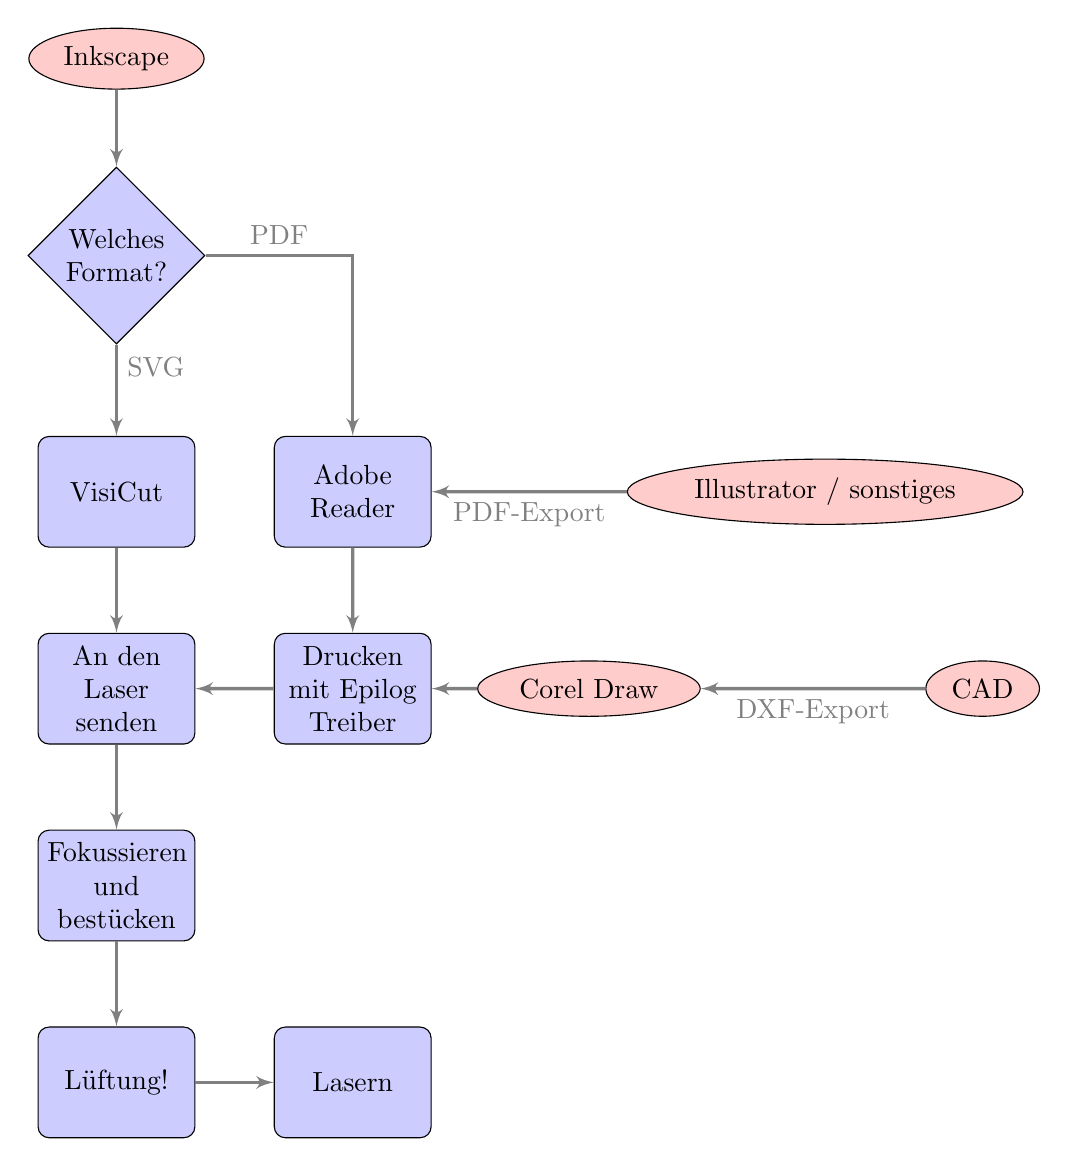
\begin{tikzpicture}[scale=0.8, node distance = 2.5cm, auto]
	%nodes, loosely sorted bottom to top
	\node [block] (luft) {Lüftung!};
	\node [block, right of=luft, node distance=3cm] (laser) {Lasern};
	\node [block, above of=luft] (fokus) {Fokussieren und bestücken};
	\node [block, above of=fokus] (uebertragen) {An den Laser senden};
	\node [block, above of=uebertragen] (visicut) {VisiCut};
	\node [decision, above of=visicut] (i_format) {Welches Format?};
	\node [cloud, above of=i_format, node distance=2.5cm] (inkscape) {Inkscape};
	\node [block, right of=uebertragen, node distance=3cm] (drucker) {\enquote{Drucken} mit Epilog Treiber};
	\node [block, right of=visicut, node distance = 3cm] (pdf) {Adobe Reader};
	\node [cloud, right of=drucker, node distance=3cm] (corel) {Corel Draw};
	\node [cloud, right of=corel, node distance=5cm] (cad) {CAD};
	\node [cloud, right of=pdf, node distance=6cm] (anderes) {Illustrator / sonstiges};
	%paths
	%decision i_format
	\path [line] (i_format) -- node [near start] {SVG} (visicut);
	\path [line] (i_format) -| node [near start] {PDF} (pdf);
	%inkscape
	\path [line] (inkscape) -- (i_format);
	%luft
	\path [line] (luft) -- (laser);
	%fokus
	\path [line] (fokus) -- (luft);
	%anderes
	\path [line] (anderes) -- node {PDF-Export} (pdf);
	%visicut
	\path [line] (visicut) -- (uebertragen);
	%pdf
	\path [line] (pdf) -- (drucker);
	%cad
	\path [line] (cad) -- (corel) node[midway,below] {DXF-Export};
	%corel
	\path [line] (corel) -- (drucker);
	%drucker
	\path [line] (drucker) -- (uebertragen);
	%uebertragen
	\path [line] (uebertragen) -- (fokus);

\end{tikzpicture}

%alte Version, gefällt mir grad nicht mehr
%\begin{tikzpicture}[scale=2, node distance = 2cm, auto]
%    % Place nodes
%	\node [block] (idee) {Idee};
%    \node [decision, below of=idee] (ready?) {Zeichung schon fertig?};
%    \node [decision, left of=ready?] (format) {Format?};
%    \node [decision, right of=ready?] (diy) {Pogramm?};
%    \node [block, below of=diy] (inkscape) {Zeichnung in Inkscape erstellen};
%    \node [block, right of=diy] (corel) {Zeichnung in Corel erstellen};
%    \node [block, below of=corel] () {}
%    % Draw edges
%    \path [line] (idee) -- (ready?);
%	\path [line] (ready?) -- node [near start] {Ja} (format);
%	\path [line] (ready?) -- node [near start] {Nein} (diy);
%\end{tikzpicture}

\section{Stempel herstellen}
\label{stempel}
Mit dem Lasercutter lassen sich auch gut Stempel herstellen.
Dafür gibt es im FabLab speziellen Stempelgummi.
Dieser lässt sich mit dem Laser tief gravieren und ausschneiden.

Eine genaue Anleitung dazu gibt es unter \url{https://fablab.fau.de/project/stempel}.

\section{Lessons Learned}

\subsection{Boxen automatisch generieren lassen}

Die Vektordaten für eine praktische Box muss man nicht selbst erzeugen. Am einfachsten geht es, wenn man einen web-basierten Gerneratoren verwendet. \\

Bisher wurden gute Erfahrungen mit folgenden Seiten gemacht:
\begin{itemize}
	\item \url{http://www.makercase.com/} \\
		Wird als Vektorgrafik ausgegeben. Pfade sind so angeordnet, dass der Laser nahe beieinanderliegende Pfade nacheinander bearbeitet (gut, da ansonsten viel Zeit durch das Verfahren des Lasers verbraucht wird) \\
		\textbf{Achtung!} Dimensionen werden immer als outside-Dimensionen berechnet. Auswahl \enquote{innerside} wird nicht berücksichtigt.
	\item \url{http://boxdesigner.connectionlab.org/} \\
		Wird als PDF ausgegeben. Allerdings ist (wenn nicht Visicut verwendet wird) die Abfolge der Pfade eher zufällig. Somit entstehen zusätzliche Zeiten durch das Verfahren des Lasers.
\end{itemize}


\subsection{Schnittmuster platzsparend anordnen}
Je nach Design kann Platz gespart werden, wenn auszuschneidende Objekte
\enquote{ineinander} geschoben werden.
Diese mühselige Aufgabe kann von verschiedenen Programmen übernommen werden.
Beispiele sind \url{https://svgnest.com/} (im Browser) oder \url{https://deepnest.io/} (zum Installieren).


\newpage
\section{Hinweise für Betreuer: Wartung - LTT iLaser}
In Härtefällen, z.\,B. wenn ein kompletter Auftrag fehlgeschlagen ist, können von einem Betreuer die Kosten für die Laufzeit gemindert oder erlassen werden.

\textbf{Achtung! Mache folgendes nur, wenn du wirklich Ahnung hast -- Fehler können teuer werden!}

Normale Reinigung der Optik und Mechanik siehe Benutzerhandbuch des Herstellers. Problembehandlung siehe Wartungshandbuch des Herstellers. Beides liegt auf der Dateifreigabe unter Fablab / Geräte / Laser.

\todo{...}

\newpage
\section{Hinweise für Betreuer: Wartung - Epilog Zing}

\textbf{Achtung! Mache folgendes nur, wenn du wirklich Ahnung hast -- Fehler können teuer werden!}

\subsection{wöchentliche Reinigung: Linse, Spiegel, Wagen}
\begin{itemize}
\label{linsenreinigung}
 \item Auf den Schneidetisch etwas weiches legen, z.\,B. ein Stück altes Sweatshirt oder eine ausgebreitete Zeitung.
 \item ggf. Schneidetisch runterfahren
 \item Linse herausschrauben, entnehmen und mit der Gewinde-Seite nach unten auf den Tisch legen.
 \item 3-5 Tropfen Linsenreiniger auf Wattestäbchen aufbringen. Nur den originalen Reiniger verwenden, dieser ist 25 Prozent Isopropanol in demineralisiertem Wasser gelöst.
 \item vom Mittelpunkt nach außen wischen, dabei das Stäbchen immer ganz leicht weiterdrehen, niemals zurückdrehen! Dreck darf nicht in die Beschichtung gekratzt werden!
 \item Dies wiederholen, bis die Linse sauber aussieht. Dabei jedes mal eine frische Seite des Wattestäbchens und neuen Linsenreiniger verwenden!
 \item Nun ein letztes mal im Zickzack die ganze Fläche abwischen.
 \item Linse vollständig trocknen lassen und wieder einbauen.
 \item Mit dem Spiegel ebenso verfahren, normalerweise ist er allerdings sauber und muss nicht geputzt werden.
\end{itemize}

% TODO
\subsection{Wartung der Mechanik}
%TODO  fertig machen
Der Schneidtisch läuft auf 4 Gewindestangen. Diese müssen von Zeit zu Zeit gereinigt werden. Dazu saugt man den Innenraum und die Stangen ab und wischt mit einem alten Lappen nach. Wichtig ist, dass an den Lagern sich keine Staubklumpen sammeln. Auf die staubfreien Stangen gibt man wenige Tropfen Öl.
%TODO Skizze der Filteranlage
\subsubsection{Filtermatte wechseln}
Für den Holzkasten-Filter wird eine Filtermatte F5 auf 50x66cm zurecht geschnitten.
Wechsel: seitliche Verschlüsse öffnen, Deckel abnehmen, Filtermatte entfernen, neue Matte mit flauschiger Seite nach oben einlegen, Kasten schließen.

Dieser Filter ersetzt die folgenden Unterkapitel. (Diese werden nur noch für den Messebetrieb benötigt.)
\subsubsection{Grobfilter wechseln}
Der Grobstaubfilter ist die Tasche auf der linken Seite. Im neuen Zustand ist er weiß. Gewechselt werden muss der Filter, sobald die Anlage wegen zu geringem Durchsatz abschaltet. Dann ist der Filter meist braun.

Der Filter ist mit einem eingesteckten Gummistutzen an der Rückwand befestigt. Dieser kann einfach durch leichtes Hin und Her drehen abgezogen werden. Wichtig ist beim Wechsel nicht auf den Filter zu drücken, um ein unnötiges Stauben zu vermeiden. Sobald der Filter ausgebaut ist, schraubt man die Rohrschelle auf und trennt den Stoffteil zur Entsorgung ab. Auf das schwarze Kunststoffstück wird eine neue Tasche aufgezogen und mit der Rohrschelle befestigt.

Zum Schluss wird der Filter wieder eingesteckt. Ein Grobfilterwechsel sollte zusammen mit dem Stand der Lüftungslaufzeit im Laserlogbuch vermerkt werden. (siehe Wiki-Seite des Lasers)
\subsubsection{HEPA-Filter wechseln}
\label{subsubsec:HEPA-Filter}
Der Feinstaubfilter besteht aus zwei Teilen. Der obere mit Klammern befestigte Teil ist der HEPA-Filter. Der Verband aus beiden Filtern kann durch Herunterklappen des weißen Hebels und Herausziehen des schwarzen Kastens aus der Anlage entfernt werden.
Der HEPA-Filter muss nur sehr selten gewechselt werden. Dies erkennt man daran, dass die Lamellen sehr \enquote{pelzig} aussehen. \emph{Achtung! Die Lamellen sind sehr empfindlich und dürfen nicht berührt werden.}
Ein Wechsel des HEPA-Filters muss im Laserlogbuch zusammen mit dem Stand der Anlagenlaufzeit notiert werden.
\subsubsection{Aktiv-Kohle-Filter wechseln}
Der Aktiv-Kohle-Filter ist der schwarze Kasten unter dem HEPA-Filter. Zum Ausbau siehe den Abschnitt \ref{subsubsec:HEPA-Filter}.

Zunächst sollte man nach dem Ausbau die untere Gummidichtung überprüfen. Diese schließt den Filter luftdicht ab und verschleißt von Zeit zu Zeit. Defekte Stellen sollten heraus geschnitten werden und durch neues P-Klebeband von Tesa Moll ersetzt werden. Dieses Band lässt sich über unser Teilesystem finden. Dabei sollten zwei Bänder so nebeneinander geklebt werden, dass sich ein Hohlraum zwischen zwei Wülsten bilden kann.

Bei schlechter Filterleistung (Geruchsbildung) ist es oft ausreichend, die Aktivkohle neu aufzuschütteln. Danach kann es vorkommen, dass die Lüftung etwas Staub spuckt, also erstmal draußen betreiben.

Wenn dies nichts bringt, muss die Aktivkohle gewechselt werden. Dazu entfernt man das schwarze Klebeband am oberen Rand des Filters. Dieses sollte man aufheben, da es wieder verwendet werden kann. Für die weiteren Schritte sollte nach Außen gegangen werden. Zunächst entfernt man den Deckel, welcher mit vier Ausstülpungen des Grundteiles befestigt ist. Jetzt werden die Aktiv-Kohle und die zwei Filtermatten entsorgt. Achtung! Dies staubt massiv. Den Staub nicht einatmen!

Abschließend legt man eine Filtermatte in den Boden, gibt die Aktiv-Kohle darauf und legt eine Filtermatte in den Deckel. Den Deckel wieder festdrücken und mit Klebeband luftdicht verschließen. Eventuelle Lücken werden mit weiterem Klebeband gedichtet. Nun montiert man den HEPA-Filter und schiebt die Einheit wieder in die Absauganlage.
Ein Wechsel des Aktiv-Kohle-Filters muss im Laserlogbuch zusammen mit dem Stand der Anlagenlaufzeit notiert werden.
\subsubsection{Neue Grobfilter nähen}
Das Material für die Filter kann bei Großhändlern quadratmeterweise bestellt werden. Das Schnittmuster gibt es im Netzlaufwerk. Beim Nähen ist es wichtig auf eine dichte Naht (Stiche nah beieinander, eventuell Overlock) zu achten. Außerdem muss man aufpassen, dass die Öffnung groß genug für den Gummistutzen ist.
\subsection{Lasergitter reinigen}
Durch verbrannte Holz und Acrylreste verfärbt sich das Metallgitter des Lasertisches immer weiter. Ab einem gewissen Grad färbt dieser Schmutz ab. Wenn dies eintritt muss das Gitter gereinigt werden.
\begin{itemize}
	\item Gitter herausnehmen (mit Rahmen) und am Waschbecken bereit legen. Backofenreiniger und Heißluftpistole hohlen.
	\item Mit der Heißluftpistole das Gitter gut aufheizen. (Richtig heiß machen, jedoch nicht so heiß, dass der Lack sich ablöst!)
	\item Backofenspray schütteln und gleichmäßig von allen Seiten auftragen.
	\item Mit der Heißluftpistole weiter aufheizen. Achtung! Geruchsentwicklung! Absaugung des Raumes laufen lassen.
	\item Gegebenenfalls Prozedur wiederholen.
	\item Mit viel Wasser und wenig Sauerei ausspülen.
	\item Zwischen den Gitterblechen kann mit einem Pfeifenreiniger oder einem Tuch gewischt werden. Achtung! Das Blech lässt sich leicht verbiegen.
	\item Zum Schluss den Boden des schwarzen Gehäuses auswischen. Dabei die Hand sehr flach machen und nicht an den Gitterkanten schneiden!
	\item Gut durchtrocknen lassen und wieder einbauen. Dabei auf Ebenheit achten.
\end{itemize}
\subsection{ausführliche Wartung}
%TODO
Zur ausführlichen Wartung gehören die folgenden Punkte:
\begin{itemize}
\item Ausbauen des Schlittens
\item Abwischen der Laufflächen des Schlittens (das Profil und die Rollen mit einem weichen Lappen reinigen)
\item Prüfen der Riemenspannung von X- und Y-Achse
\item Reinigen der Linse und Überprüfen auf Defekte
\item Reinigen des Innenraums mit Breff Eingebrannte oder mit Industriereiniger
\item Reinigen und Abrichten des Gittertisches
\item Wartung der Z-Mechanik
\item Warten der Filtereinheit
\item Zerlegen des Absaugkasten und Ausblasen des Saugermotors
\item weiteres siehe Wartungsliste
\end{itemize}

\subsection{Lasermatch einstellen}
Der Lasercutter graviert die Zeilen immer abwechseld von links nach rechts und umgekehrt. Dabei kann ein leichter Versatz zwischen links- und rechtsherum gravierten Zeilen auftreten, der vertikale Gravurkanten kammförmig erscheinen lässt. Zum Testen lasert man mit 1000dpi eine feine vertikale Linke oder feine Schrift (ein kleines i in 9pt Times). Dies wiederholt man mit verschiedenen Lasermatch-Einstellungen und wählt die, bei der die Kante optimal aussieht.

Details dazu stehen im Handbuch.



\section{\nurLTT Fehlerbehebung}
In diesem Abschnitt geht es um die Beseitigung häufiger Fehler. Wenn das Werkstück fehlgeschlagen ist, werden die Laserzeitkosten des Fehlschlags in der Regel erlassen. Material muss weiterhin bezahlt werden.

\todo{...}


\section{\nurZing Fehlerbehebung}
In diesem Abschnitt geht es um die Beseitigung häufiger Fehler. Wenn das Werkstück fehlgeschlagen ist, werden die Laserzeitkosten des Fehlschlags in der Regel erlassen. Material muss weiterhin bezahlt werden.

\subsection{Windows-Druckertreiber}
\subsubsection{Objekt wird nicht geschnitten, sondern graviert}
\begin{itemize}
 \item Liniendicke 0.1 \textbf{Pixel} bzw. Haarlinie (Corel)
 \item Inkscape: Deckkraft 100\% (Objekt $\rightarrow$ Füllung und Kontur $\rightarrow$ Schieberegler ganz unten: Deckkraft)
 \item Keine Transparenz (Alphakanal, Deckkraft) verwenden! Auch nicht in Farbverläufen.
 \item Illustrator: Gruppen mit Zuschneidepfad machen oft Probleme; diese auflösen.
 \item Richtiges Programm verwendet? Siehe Abschnitt \ref{ArbeitsablaufFlowchart} Arbeitsablauf
 \item PDFs werden beim Exportieren manchmal gerastert bzw. kaputtgemacht. Keinen PDF-Export aus Corel verwenden!
\end{itemize}


\subsubsection{Probleme mit 1000dpi}
Verwendet man die Einstellung 1000dpi können Fehler auftreten. Meist hängt der Druckjob ewig fest oder die Data-Leuchte geht nicht mehr aus. Dieses Problem lässt sich nur durch Neustarten aller Geräte lösen. Also zuerst die VM neustarten, dann den Lasercutter. Der Druckjob muss erneut geschickt werden. Jetzt sollten entweder 500dpi genutzt werden oder VisiCut.

\subsubsection{Data leuchtet ständig, Job hält an}
Data soll vor dem Starten eines Jobs ausgegangen sein! Ansonsten hält der Job manchmal irgendwann in der Mitte an.

Das bedeutet, dass Windows sich verschluckt hat und den Rest des Jobs nicht senden will. Stop drücken, eine Epilog-Gedenkminute lang warten und beten, dass Data spontan ausgeht. Ansonsten auf die harte Tour: Stop, Reset, ggf. den Nullpunkt markieren damit man ihn wiederfindet. Laser ausschalten, Druckauftrag abbrechen (in der Windows-VM über das Druckersymbol in der Taskleiste), Windows-VM über Startmenü neustarten, Laser wieder anschalten.

\subsection{Mechanik}
Bitte führe Wartungen an der Mechanik nur dann durch, wenn du weißt, was du tust!

\subsubsection{Gravur zittrig}
\begin{wrapfigure}{r}{2cm}
  \vspace{-50pt} %WORKAROUND: Nicht so viel leerer weißer Platz
  \includegraphics[width=2cm]{./img/fehler-umlenkspiegel.png}
  \vspace{-20pt} %WORKAROUND: Nicht so viel leerer weißer Platz
\end{wrapfigure}
 Wenn es so aussieht wie auf dem Bild: Umlenkspiegel und Linse festschrauben.

\subsubsection{Fokusprobleme}
Ein falscher Fokus äußert sich dadurch, dass das Schneiden schlecht und die Gravur nur schwach und verrauscht funktioniert. Prüfe zuerst mit dem Fokuspendel, ob der Fokus richtig eingestellt ist.

Wenn es trotzdem nicht funktioniert, kann es sein dass die Länge des Fokuspendels nicht mehr stimmt. Dies kann mit einem Test überprüft werden:

Zum Testen wird VisiCut gestartet und ein spezielles LaserScript geladen: Datei \pfeil Beispiele \pfeil vordefiniert \pfeil LaserScript \pfeil Focustest und auf \enquote{Papier 80g, alles cut} gestellt.
Als nächste muss ein A3 Blatt Papier im Querformat (oder 2x A4 nebeneinander) eingelegt und auf die Materialoberseite fokussiert werden.

Das Script testet auf dem Papier verschiedene Fokusabstände und wenn der Fokus so wie eingestellt stimmt, sollte der dünnste, präzieseste Schnitt bei Höhe 0 vorliegen.


\subsubsection{Material wird in einer Ecke nicht durchtrennt}
Es kann vorkommen, dass Material in einer der Ecken nicht richtig durchtrennt wird trotz richtig eingestelltem Fokus. Dies liegt meistens daran, dass der Tisch schief steht.

Zur Behebung wird der Tisch ausgebaut. (Dazu den Arm bei ausgeschaltenem X/Y aus dem Weg schieben.) Meist liegt etwas in einer der beiden Vertiefungen der unteren Lineale. Diese gegebenenfalls reinigen. Zum Abschluss den Tisch wieder gerade einsetzen, sicher stellen, dass er in den Vertiefungen sitzt und mit sanftem Druck bis zum Boden drücken.

\subsubsection{Wagen macht schabende Geräusche}
Der blaue Wagen läuft auf drei Rollen im schwarzen Arm. Falls der Wagen nicht korrekt eingesetzt ist, lässt er sich nur schwergängig unter schabenden Geräuschen bewegen. Um dies zu beheben drückt man die Klammer, die das Rad auf der dem Benutzer abgewandten Seite hält zusammen. Jetzt lässt sich der Wagen bewegen. Eigentlich müsste er die richtige Position \enquote{von selbst} finden. Eventuell ist auch der Metallträger, der am Riemen befestigt ist im Arm verklemmt. Um dies zu beseitigen, löst man die zwei Schrauben auf dem Wagen, die den Träger fest halten und montiert die Anlage neu.

\subsection{Laserröhre}
\subsubsection{unterbrochene Schnittkanten}
Wenn der Laser zu heiß wird, scheint er einfach den Strahl für einen kurzen Moment abzuschalten. Dies zeigt sich dann in einer mehrfach unterbrochenen Schnittlinie. Die einzelnen \enquote{Wiedereinstiche} liegen dabei direkt nebeneinander. Eine Lösung scheint zu sein, sicherzustellen, dass der Laser auf der linken Seite kühle Luft ansaugt und dort kein Dreck ist.
\subsubsection{Leistungseinbrüche}
Wenn der Laser für ein vernünftiges Ergebnis deutlich höhere Leistungseinstellungen als gewöhnlich benötigt, ist das ein Hinweis auf eine verschmutzte Linse. Nach Abschalten des roten Lasers, kann man den Verschmutzungsgrad der Linse mit einem Spiegel überprüfen. Die Reinigungsprozedur ist in \ref{linsenreinigung} auf Seite \pageref{linsenreinigung} beschrieben. Bei schlechten Lichtverhältnissen kann es auch sein, dass eine Verschmutzung erst nach Ausbau der Linse erkennbar ist.
\subsubsection{Müdigkeit}
Wenn der Laser mehrere Tage nicht genutzt wird, ist er in der ersten halben Stunde etwas müde -- wahrscheinlich ist die Ionisierung der Laserröhre dann noch nicht so gut. Die Röhre hat dann manchmal Probleme zu zünden, sodass manche Stellen nicht oder nur teilweise gelasert werden. Nach etwas Benutzung verschwindet das Problem von selber.


\newpage
\ccLicense{lasercutter-einweisung}{Einweisung Lasercutter}

\end{document}
